%\textsl{}%!TEX TS-options = --shell-escape
%!TEX TS-program = pdflatex
\documentclass[%
   10pt,              % Schriftgroesse
   ngerman,           % wird an andere Pakete weitergereicht
   a4paper,           % Seitengroesse
   DIV11,             % Textbereichsgroesse (siehe Koma Skript Dokumentation !)
]{scrartcl}%     Klassen: scrartcl, scrreprt, scrbook, article
% -------------------------------------------------------------------------

\usepackage[utf8]{inputenc} % Font Encoding, benoetigt fuer Umlaute
\usepackage[english]{babel}   % \textsl{}Spracheinstellung

\usepackage[T1]{fontenc} % T1 Schrift Encoding
\usepackage{textcomp}    % Zusatzliche Symbole (Text Companion font extension)
\usepackage{lmodern,dsfont}     % Latin Modern Schrift
\usepackage{dsfont}
%\usepackage{wasysym}
\usepackage{ulem}
\usepackage{graphicx}
\usepackage{eurosym}
%\usepackage{txfonts}
\usepackage{stmaryrd}
\usepackage{amsfonts}
\usepackage{amsmath}
\usepackage{hyperref}
\usepackage{tikz}
\usepackage{multirow}
\usepackage{listings}
\usepackage{etextools}
\usepackage{ifthen}
%\usepackage{TikZ} %phylogenetischer Baum
%\usetikzlibrary{calc, shapes, backgrounds} %für die Phylogenetische bäume
%\usetikzlibrary{automata,arrows}
\usepackage{subfigure} 


% Definition des Headers
\usepackage{geometry}
\geometry{a4paper, top=3cm, left=3cm, right=3cm, bottom=3cm, headsep=0mm, footskip=0mm}
\renewcommand{\baselinestretch}{1.3}\normalsize

\def\header#1#2#3#4#5#6#7{\pagestyle{empty}
\noindent
\begin{minipage}[t]{0.6\textwidth}
\begin{flushleft}
\textbf{#4}\\% Fach
#6\\% Semester
Tutor: #2  % Tutor 
\end{flushleft}
\end{minipage}
\begin{minipage}[t]{0.4\textwidth}
\begin{flushright}
\points{#7}% Punktetabelle
\vspace*{0.2cm}
#5%  Names
\end{flushright}
\end{minipage}

\begin{center}
{\Large\textbf{ Blatt #1}} % Blatt

{(Abgabe am #3)} % Abgabedatum
\end{center}
}

\newenvironment{vartab}[1]
{
    \begin{tabular}{ |c@{} *{#1}{c|} } %\hline
}{
    \end{tabular}
}

\newcommand{\myformat}[1]{& #1}

\newcommand{\entry}[1]{
  \edef\result{\csvloop[\myformat]{#1}}
  \result \\ \hline
}

\newcommand{\numbers}[1]{
  \newcounter{ctra}
\setcounter{ctra}{1}
\whiledo {\value{ctra} < #1}%
{%
  \myformat{\thectra}
  \stepcounter{ctra}%
}
\myformat{\thectra}
}
\newcommand{\emptyLine}[1]{
  \newcounter{ctra1}
\setcounter{ctra}{1}
\whiledo {\value{ctra1} < #1}%
{%
  \myformat{\hspace*{0.5cm}}
  \stepcounter{ctra1}%
}
}

\newcommand{\points}[1]{
\newcounter{colmns}
\setcounter{colmns}{#1}
\stepcounter{colmns}
  \begin{vartab}{\thecolmns}
    \numbers{#1} & $\sum$ (10)\\\hline
    \emptyLine{\thecolmns}\\
  \end{vartab}
}

\begin{document}
%\header{Blatt}{Tutor}{Abgabedatum}{Vorlesung}{Bearbeiter}{Semester}{Anzahl Aufgaben}
\header{10}{Alexander Seitz}{18. January 2016}{Bioinformatics I}{\\Jonas Ditz \\\& Benjamin Schroeder}{WS 15/16}{2}

\section*{Theoretical Assignment - \textit{Assembly using de Bruijn graph}}

The de Bruijn graph for the reads provided on the assignment sheet would look like the graph in
Figure \ref{fig:4mere}, if one chooses $k = 4$. As one can see easily, there are not just one but 
four different Eulerian paths in the graph. Each path results in one of the following superstring:

\begin{align}
 S_1 &= ACCGTTAACGTAAACGT \nonumber \\
 S_2 &= ACCGTAAACGTTAACGT \nonumber \\
 S_3 &= ACCGTTAAACGTAACGT \nonumber \\
 S_4 &= ACCGTAACGTTAAACGT \nonumber
\end{align}

This happens due to the fact that there are nodes with more than one outgoing an incoming edge. If
one chooses $k = 5$ the resulting de Bruijn graph would look like the graph in Figure \ref{fig:5mere}.
It is obvious that the number of nodes is depended on $k$. With a bigger $k$ there are more nodes in 
the resulting de Bruijn graph. The resulting graph for $k = 5$ is non-connected. So the superstring 
for this graph is not just one but three strings: 

\begin{align}
 S_{part_1} &= TAAACTG \nonumber \\
 S_{part_2} &= CGTAACGTTAA \nonumber \\
 S_{part_3} &= ACCGT \nonumber
\end{align}

One can see that $S_{part_1} = f_5$ and $S_{part_3} = f_1$, while $S_{part_2}$ is the result of an 
overlap alignment between $f_2$, $f_3$ and $f_4$. In general the second graph is more realistic. 
It is very unlikely to get a connected graph with real-life data. So it is possible that just $f_2$, 
$f_3$ and $f_4$ come from the same area in the target DNA. $f_1$ and $f_5$ could come from a different 
contig and, hence, result in this graph (Figure \ref{fig:5mere}). Since this is a minimal example 
the first graph (Figure \ref{fig:4mere}) is not wrong but one should not expect to get a connected 
graph all the time. In fact a connected graph is suspicious, normally.

\begin{figure}[h]
 \centering
 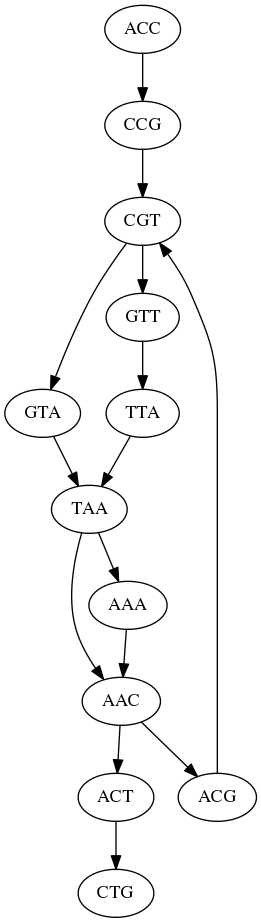
\includegraphics[width=1\textwidth]{deBruijnGraph_4mere.png}
 \caption{De Bruijn graph for the given reads and $k = 4$.}
 \label{fig:4mere}
\end{figure}

\begin{figure}[h]
 \centering
 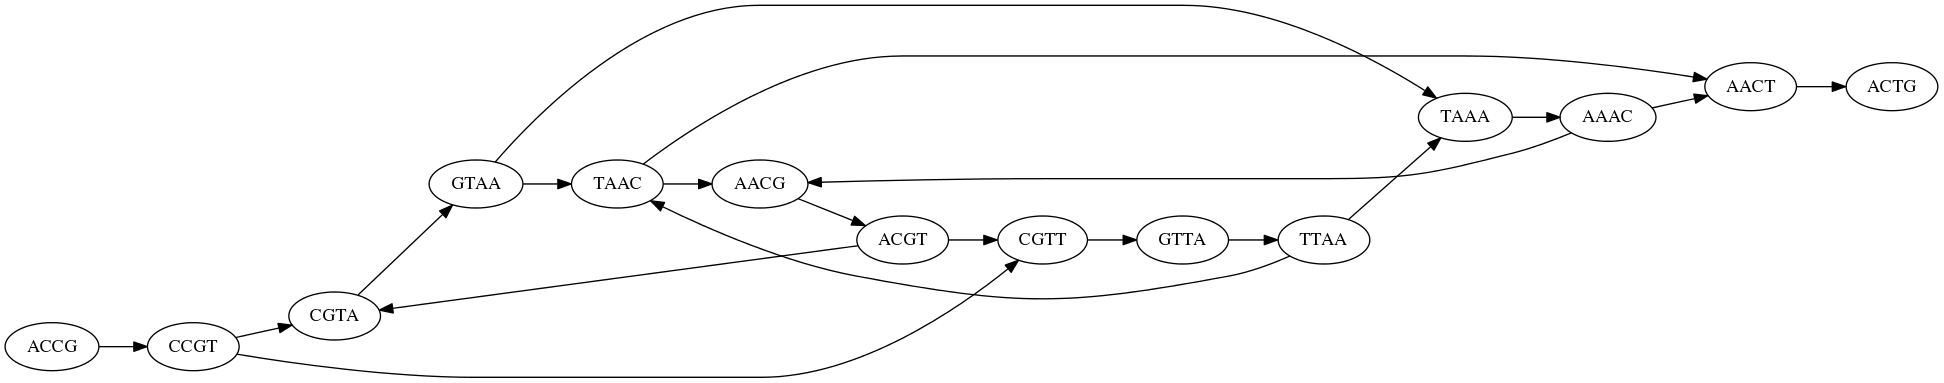
\includegraphics[width=1\textwidth]{deBruijnGraph_5mere.png}
 \caption{De Bruijn graph for the given reads and $k = 5$.}
 \label{fig:5mere}
\end{figure}



\section*{Practical Assignment - \textit{Assemble the human mitochondrial genome}}

\end{document}